\documentclass[tikz,border=3mm]{standalone}
\begin{document}
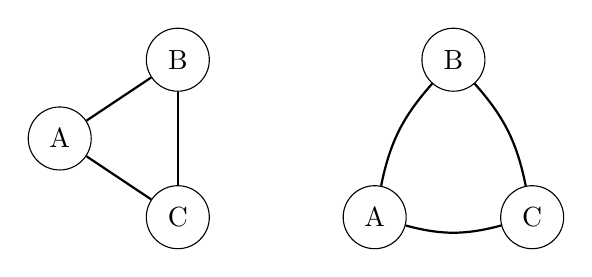
\begin{tikzpicture}[
    node/.style={circle, draw, minimum size=8mm}, % Стиль для узлов
    straight/.style={thick}, % Стиль для прямых рёбер
    curved/.style={thick, bend left=15} % Стиль для округлых рёбер
]

    % Первый граф (прямые рёбра)
    \begin{scope}[xshift=-2cm] % Сдвигаем первый граф влево
        % Узлы
        \node[node] (A1) at (0, 0) {A};
        \node[node] (B1) at (1.5, 1) {B};
        \node[node] (C1) at (1.5, -1) {C};

        % Рёбра
        \draw[straight] (A1) -- (B1);
        \draw[straight] (A1) -- (C1);
        \draw[straight] (B1) -- (C1);
    \end{scope}

    % Второй граф (округлые рёбра)
    \begin{scope}[xshift=2cm] % Сдвигаем второй граф вправо
        % Узлы
        \node[node] (A2) at (0, -1) {A};
        \node[node] (B2) at (1, 1) {B};
        \node[node] (C2) at (2, -1) {C};

        % Рёбра
        \draw[curved] (A2) to (B2);
        \draw[curved] (C2) to (A2);
        \draw[curved] (B2) to (C2);
    \end{scope}

\end{tikzpicture}
\end{document}